% step_plot/2017-201_ndvi.pdf 
% step_plot/2017-202_itpl.pdf 
% step_plot/2017-203_itpl_rew.pdf 
% step_plot/2017-204_ndvi_scl.pdf 
% step_plot/2017-205_show_res.pdf 
% step_plot/2017-206_corr.pdf 
% step_plot/2017-207_uncert.pdf 
% step_plot/2017-208_corr_itpl_rew.pdf

\begin{figure*}[!h]
	% \vspace{-15pt}
	% \centering
	% \begin{subfigure}[b]{0.42\textwidth}
	% 	\centering
	% 	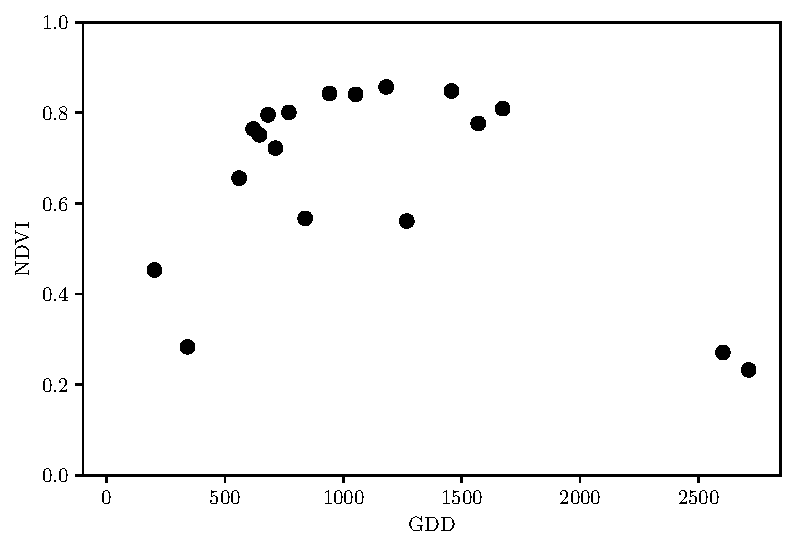
\includegraphics[width=\textwidth]{step_plot/2017-201_ndvi.pdf}
	% 	\vspace{-20pt}
	% 	\caption[NDVI {TS} with SCL45]%
	% 	{{\footnotesize NDVI {TS} with SCL45}}    
	% 	\label{fig:step_plot/2017-201_ndvi.pdf}
	% \end{subfigure}
	% \hfill
	
	\vskip\baselineskip
	\begin{subfigure}[b]{0.42\textwidth}  
		\centering 
		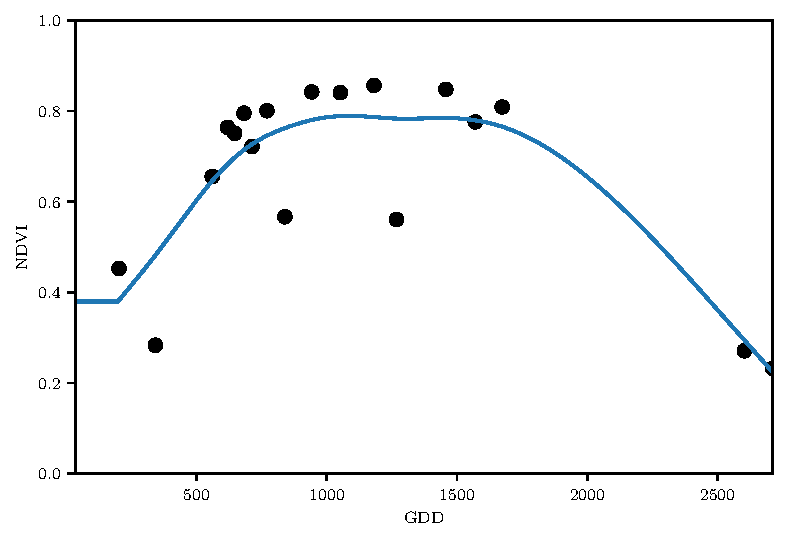
\includegraphics[width=\textwidth]{step_plot/2017-202_itpl.pdf}
		\vspace{-20pt}
		\caption[Interpolation via SS (only SCL45)]%
		{{\footnotesize Interpolation via SS (only SCL45)}}    
		\label{fig:step_plot/2017-202_itpl.pdf}
	\end{subfigure}
	% \begin{subfigure}[b]{0.42\textwidth}   
	% 	\centering 
	% 	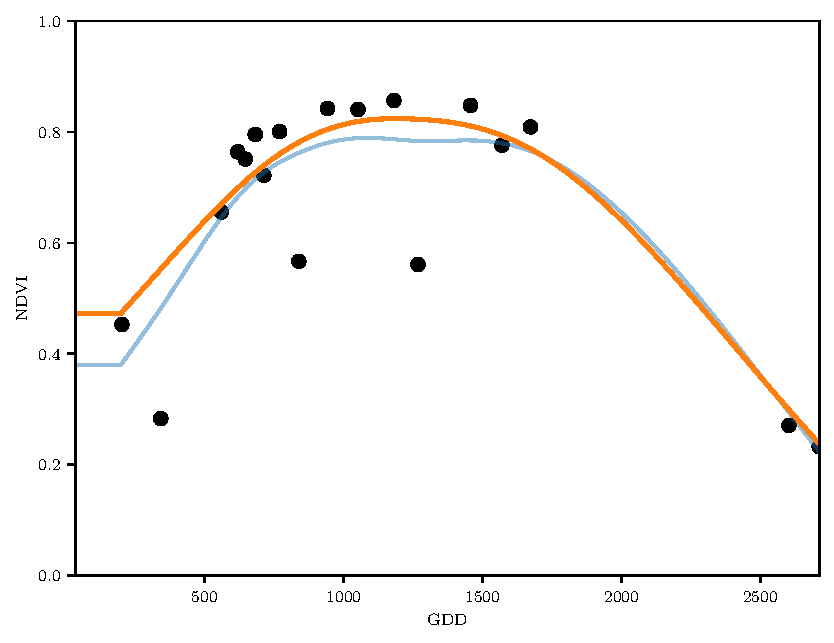
\includegraphics[width=\textwidth]{step_plot/2017-203_itpl_rew.pdf}
	% 	\vspace{-20pt}
	% 	\caption[Robustly reweighted fit]%
	% 	{{\footnotesize Robustly reweighted fit}}    
	% 	\label{fig:step_plot/2017-203_itpl_rew.pdf}
	% \end{subfigure}
	\hfill
	\begin{subfigure}[b]{0.42\textwidth}   
		\centering 
		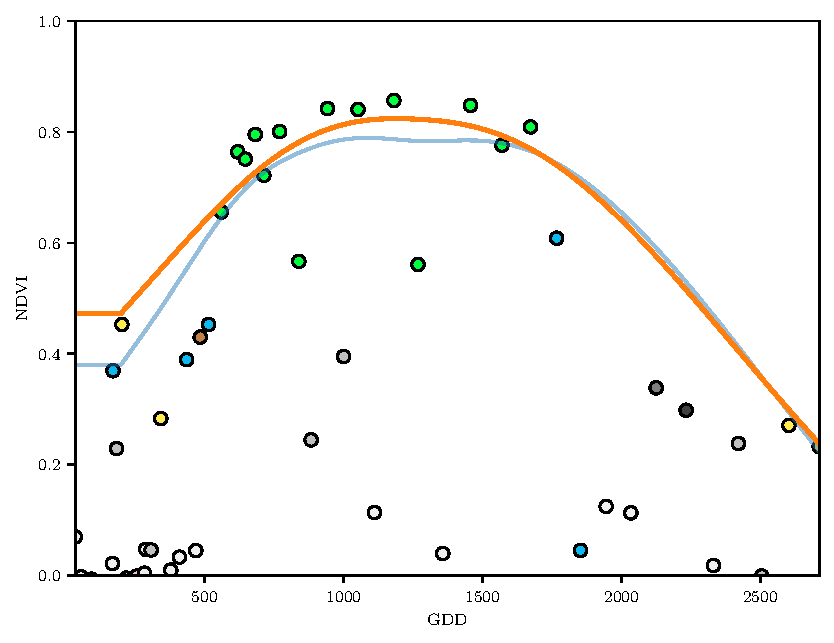
\includegraphics[width=\textwidth]{step_plot/2017-204_ndvi_scl.pdf}
		\vspace{-20pt}
		\caption[Now also consider other SCL-classes]%
		{\footnotesize Now also consider other SCL-classes}    
		\label{fig:step_plot/2017-204_ndvi_scl.pdf}
	\end{subfigure}

	\vskip\baselineskip
	\begin{subfigure}[b]{0.42\textwidth}   
		\centering 
		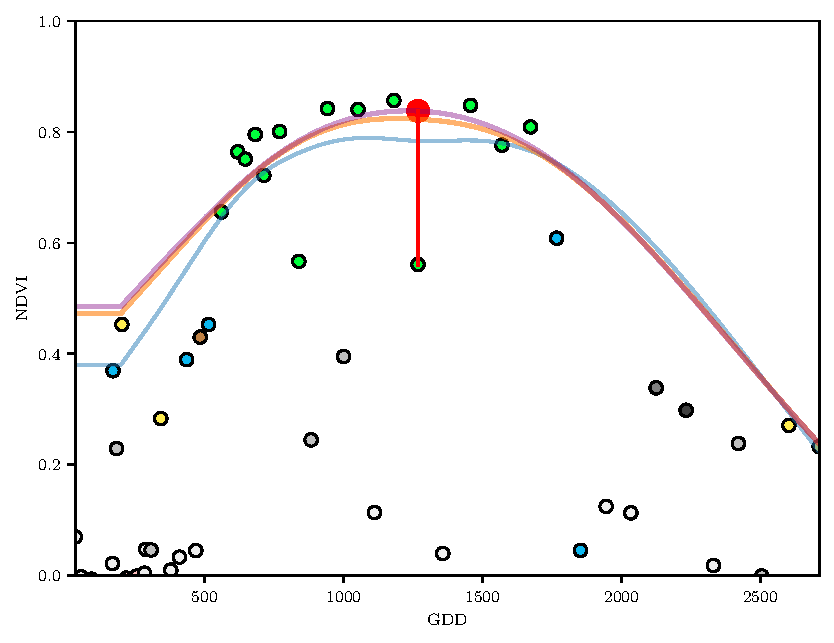
\includegraphics[width=\textwidth]{step_plot/2017-205_show_res.pdf}
		\vspace{-20pt}
		\caption[OOB estim. for each point using SCL45]%
		{{\footnotesize OOB estim. for each point using SCL45}}    
		\label{fig:step_plot/2017-205_show_res.pdf}
	\end{subfigure}
	\hfill
	\begin{subfigure}[b]{0.42\textwidth}   
		\centering 
		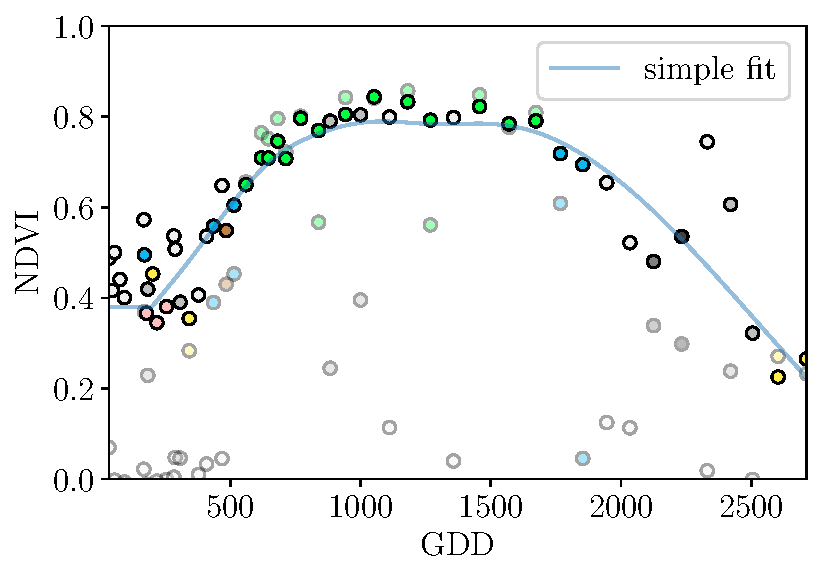
\includegraphics[width=\textwidth]{step_plot/2017-206_corr.pdf}
		\vspace{-20pt}
		\caption[Correct NDVI]%
		{\footnotesize Correct NDVI}    
		\label{fig:step_plot/2017-206_corr.pdf}
	\end{subfigure}

	\vskip\baselineskip
	\begin{subfigure}[b]{0.42\textwidth}   
		\centering 
		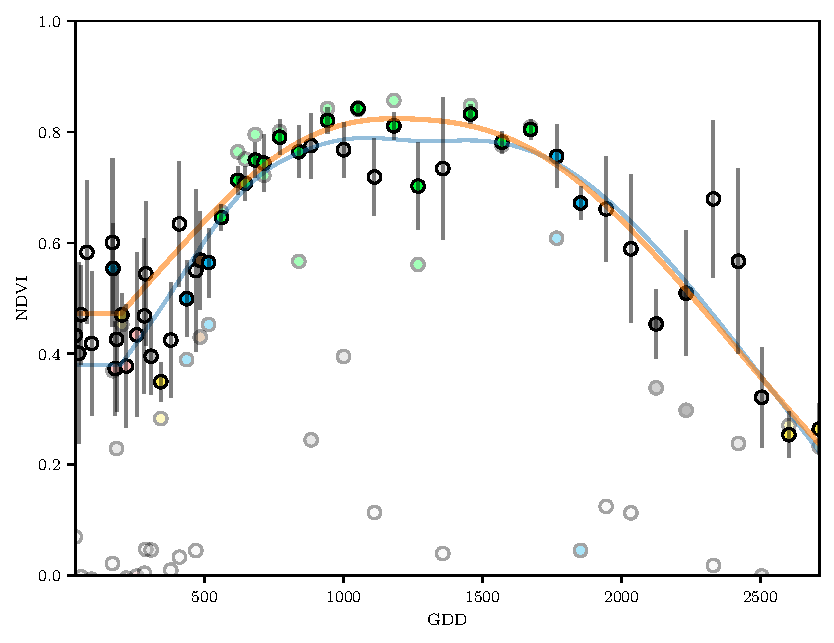
\includegraphics[width=\textwidth]{step_plot/2017-207_uncert.pdf}
		\vspace{-20pt}
		\caption[Estimate absolute errors]%
		{{\footnotesize Estimate absolute errors via statistical model}}    
		\label{fig:step_plot/2017-207_uncert.pdf}
	\end{subfigure}
	\hfill
	\begin{subfigure}[b]{0.42\textwidth}   
		\centering 
		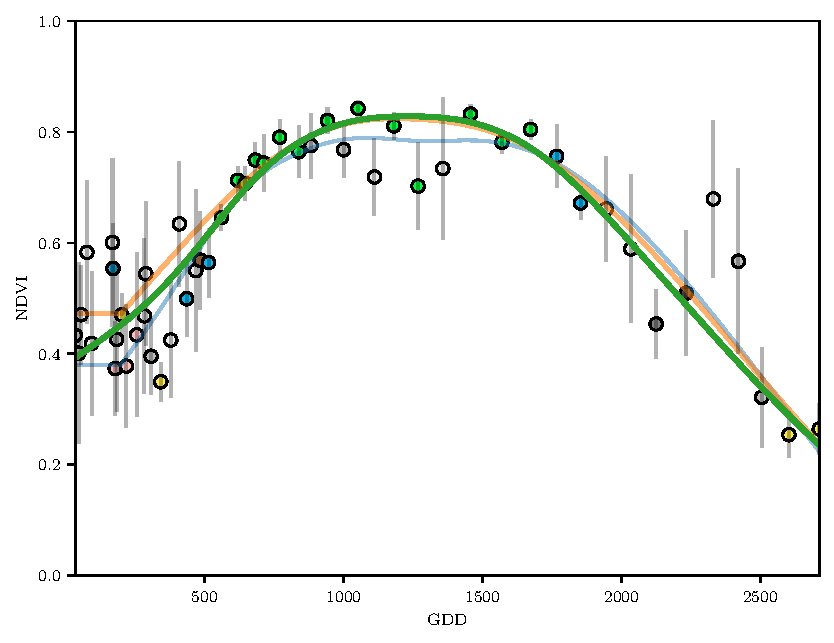
\includegraphics[width=\textwidth]{step_plot/2017-208_corr_itpl_rew.pdf}
		\vspace{-20pt}
		\caption[Interpolation (SS) on weights derived from uncertainties.]%
		{\footnotesize Robust interpolation on weights derived from uncertainties.}    
		\label{fig:step_plot/2017-208_corr_itpl_rew.pdf}
	\end{subfigure}
	\caption[Stepwise illustration of robust NDVI-Correction.]{Stepwise illustration of robust NDVI-Correction. For the color encoding of the SCL classes we refer to table~\ref{tab:satelite/scl_classes}.}
	\label{fig:step_plot_ndvi_corr}
\end{figure*}
